\documentclass[12pt]{article}
\usepackage{multicol} %multicolumns
\usepackage{siunitx} %log table stuff
\usepackage{flafter}
\usepackage{amsmath} %math stuff
\usepackage{amssymb} %math symbols
\usepackage{graphicx} %including photos
\usepackage{wrapfig} %for wrapping figure
%\graphicspath{{./Report For Titanium Doping/}} %path of folder from where photo needs to be extracted, NOT NECESSARY AT ALL TIMES
\usepackage[utf8]{inputenc}
\usepackage{float} %Using [H] command to stop picturefloating around
\usepackage{enumerate} %changing labels of lists
\usepackage{fancyhdr}
\usepackage{dsfont} %for set notations and other fancy letters
\usepackage{mathrsfs}
\usepackage[compat=1.0.0]{tikz-feynman}

\usepackage{geometry}
\geometry{
a4paper,
total={170mm,257mm},
top=20mm,
}
\usepackage{array}
\setlength\extrarowheight{4pt}
%\usepackage[dvipsnames]{xcolor} %for using coloured text
\usepackage{longtable,pdflscape,booktabs} % long table stuff
\usepackage{lscape} 
\usepackage{caption}
\captionsetup{labelformat=empty}
\captionsetup[subfigure]{labelformat=empty}
\usepackage{subcaption}
\usepackage{setspace} %for desired spacing between lines
\usepackage{blindtext} % for blind text in contents page
\usepackage[normalem]{ulem} %dash and dotted underline
\usepackage{bm} % for bold math symbols- using command \boldsymbol
\usepackage{mathtools} %for rcases
\usepackage{hyperref} %for hyperlinks
\usepackage{romannum} %for Roman Numerals
\usepackage[makeroom]{cancel} % for striked out or other stuff in math environment
\usepackage{tikz}
\usepackage{empheq} %  fancy math stuff
\usepackage{xfrac}
\usepackage{fancybox} %for fancy boxes
\usepackage{circuitikz}
\usepackage{listings}

\allowdisplaybreaks
\colorlet{linkequation}{blue} %making coloured equation refernces

\usetikzlibrary{shadows} %defines shadows
\usepackage[framemethod=tikz]{mdframed}
\usepackage{tcolorbox} %coloured boxes

\tikzset{rndblock/.style={rounded corners,rectangle,draw,outer sep=1pt,inner sep=5pt,line width=1pt}}

% Command Definition
% 1 optional to customize the aspect, 2 mandatory: text to be framed
\newcommand{\mybox}[2][]{\tikz[baseline=(h.base)]\node[rndblock,#1] (h) {#2};}

%definining new command to make coloured equation references
\newcommand*{\myref}[1]{%
  \begingroup
    \hypersetup{
      linkcolor=linkequation,
      linkbordercolor=linkequation,
    }%
    \ref{#1}%
  \endgroup
}

%Setting equations a particular colour
\hypersetup{
colorlinks=true,
linkcolor=black,
filecolor=magenta,
urlcolor=blue,
citecolor=blue,
}

\parskip 1ex

%For circled numbers
\newcommand*\circled[1]{\tikz[baseline=(char.base)]{
            \node[shape=circle,draw,inner sep=2pt] (char) {#1};}}
            
%command for making capital roman numerals
\newcommand{\RomanNum}[1]{\MakeUppercase{\romannumeral #1}}


%%%%%%%%%%%%%%%%%%%%%%%%%%%%%%%%%%%%%%%%%%%%%%%%%%%%%%%%%%%%%%%%%%%%%%%%%%%%%%%%%%%%%%%%%%%%%%%%%%%%%%%%%%%%%%%%%%%%%%%%%%%%%%%%%%%%%%%%%%%%%%%%%%%%%%%%%%%%%%%%%%%%%%%%%%%%%%%%%%%%%%%%%%%%% DOCUMENT BEGINS %%%%%%%%%%%%%%%%%%%%%%%%%%%%%%%%%%


%\pagestyle{fancy}
%\fancyhf{}
%\fancyhead[LO]{\rightmark}
%\fancyhead[RE]{\leftmark}

\usepackage{titlesec, blindtext}
\titleformat{\section}[hang]{\Huge\bfseries}{\Roman{section}. \hspace{20pt}}{0pt}{\Huge\bfseries}

\titleformat*{\subsection}{\Large\bfseries}
\titleformat*{\subsubsection}{\large\bfseries}

\usepackage{tocloft}
\renewcommand{\cftsecleader}{\cftdotfill{\cftdotsep}}
\renewcommand{\cftsecaftersnum}{.}%

%%%%%%%%%%%%%%%%%%%%%%%%%%%%%%%%%%%%%%%%
\definecolor{codegreen}{rgb}{0,0.6,0}
\definecolor{codegray}{rgb}{0.5,0.5,0.5}
\definecolor{codepurple}{rgb}{0.58,0,0.82}
\definecolor{backcolour}{rgb}{0.95,0.95,0.92}

\lstdefinestyle{mystyle}{
    backgroundcolor=\color{backcolour},   
    commentstyle=\color{codegreen},
    keywordstyle=\color{magenta},
    numberstyle=\tiny\color{codegray},
    stringstyle=\color{codepurple},
    basicstyle=\ttfamily\footnotesize,
    breakatwhitespace=false,         
    breaklines=true,                 
    captionpos=b,                    
    keepspaces=true,                 
    numbers=left,                    
    numbersep=5pt,                  
    showspaces=false,                
    showstringspaces=false,
    showtabs=false,                  
    tabsize=2
}

\lstset{style=mystyle}
%%%%%%%%%%%%%%%%%%%%%%%%%%%%%%%%%%%%%%%%%%%%%%%%%%

\begin{document}
\doublespace
%making the title page
\pagenumbering{gobble}
\begin{titlepage}
	\begin{center}
		\vspace*{0.2cm}
		\textbf{\uline{P441/P442 - Open Lab Experiment}} \linebreak
		\vspace{1.5cm}\linebreak
		\textbf{\Large{Antenna Simulation for 21cm Hydrogen Line}}\linebreak
		\vspace{2cm} \linebreak
		\textit{Submitted By} \linebreak \textbf{ASHMITA PANDA} \linebreak 
		\textbf{ROLL NO. 1811042} \linebreak
		School of Physical Sciences \linebreak National Institute of Science, Education and Research (NISER), Bhubaneswar \linebreak
		Date of Submission : 
		\vspace{2.5cm} \linebreak
		\textit{Under the Guidance of} \linebreak \textbf{Dr. Pratap Kumar Sahoo} \linebreak Associate Professor \linebreak School of Physical Sciences \linebreak National Institute of Science Education and Research (NISER), Bhubaneswar
		\vspace{1cm} \linebreak

	\end{center}
	\begin{figure}[H]
		\centering
		
\includegraphics[width=0.17\textwidth]{niser logo}
	\end{figure}
\end{titlepage}

\raggedright
\newpage
\pagenumbering{roman}

\singlespacing
%Table of Contents
\tableofcontents
\addtocontents{toc}{~ \hfill \textbf{Page} \par}
\onehalfspacing

\newpage
\pagenumbering{arabic}
\begin{center}
	\doublespacing
	\textbf{\Large Abstract} \linebreak
	21cm Hydrogen line is one of the most useful tool of Radio Astronomy in current times. It can give us information about galaxy structures and rotation curves. It also finds applications in cosmology to probe the period from recombination to reionisation. \linebreak
  In this report, an attempt has been made to design an antenna for detecting this 21cm line. First, the theory of waveguides and antennas has been discussed. The optimum parameters have been calculated using ewa library in Matlab/Octave. The final design has been implemented using the software FEKO. 
\end{center}
\rule{17cm}{1pt}
%%%%%%%%%%%%%%%%%%%%%%%%%%%%%%%%%%%%%%%%%%%%%%%%%%%%%%%%%%%
%section - Introduction
\section{Introduction}
Antennas are one of the most widely used instrumental tool in physics. They are devices which either convert voltage from a transmitter to radio waves, or pick up radio waves from the atmosphere and convert it into voltage which can be detected by a receiver. \linebreak

In this this report, we aim to :
\begin{enumerate}[i.)]
  \item discuss the importance of the 21cm line in modern astronomy and cosmology
  \item discuss the theory of waveguides
  \item discuss properties of antennas
  \item design the antenna using FEKO 
\end{enumerate} 
%%%%%%%%%%%%%%%%%%%%%%%%%%%%%%%%%%%%%%%%%%%%%%%%%%%%%%%%%%%
%section - 21CM HYDROGEN LINE
\section{21cm Hydrogen Line}
%subsection - Theory
\subsection{Theory}
Neutral hydrogen is the most abundant element of the Universe. It is made up of one proton and one electron. 
Both the proton and electron are spin-1/2 particles. They can either be in up-spin or down-spin orientation. \linebreak

At any given point of time, the electron and proton in the neutral hydrogen atom, can either be aligned parallel to each other, or anti-parallel to each other. 
\begin{figure}[H]
  \centering
  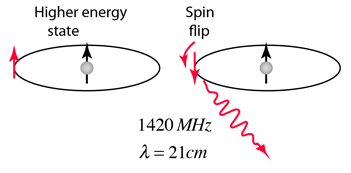
\includegraphics[width=0.5\textwidth]{Images/hflip.png}
  \caption{Fig 1. Two orientations of Neutral Hydrogen}
  \caption{\tiny Source : \url{http://hyperphysics.phy-astr.gsu.edu/hbase/quantum/h21.html}}
\end{figure}

The parallel spin state is the higher energy state compared to the anti-parallel spin state. The energy difference between the states is around 5.874eV. \linebreak

Whenever a neutral hydrogen atom goes from the parallel spin state to the anti-parallel spin state, it releases this energy in the form of a photon. This transition is called the the Spin-flip transition. \linebreak

From the Einstein-Planck equation :
\begin{equation}
  E=h \nu \label{eq:1}
\end{equation}
We can find the frequency of the emitted photon as 1420MHz. This corresponds to a wavelength of $\lambda=21$cm. 
%subsection - Importance
\subsection{Importance}
\subsubsection{In Radio Astronomy} % subsubsection 1
The 21cm line falls in the radio frequency range. It can easily penetrate the interstellar clouds and the Earth's atmosphere, thus can be observed without much interference. \linebreak

If we assume hydrogen atoms to be uniformly distributed throughout the galaxies, we should observe the 21cm line from all directions. The waves we receive will either be redshifted or blueshifted to different extents, depending on the location of their emission in the galaxy. \linebreak

We can then use this information to measure the rotation curve of our galaxy and the relative speed of each spiral arm. This information could in turn be used to indirectly calculate the mass of the galaxy. 
\begin{figure}[H]
  \centering
  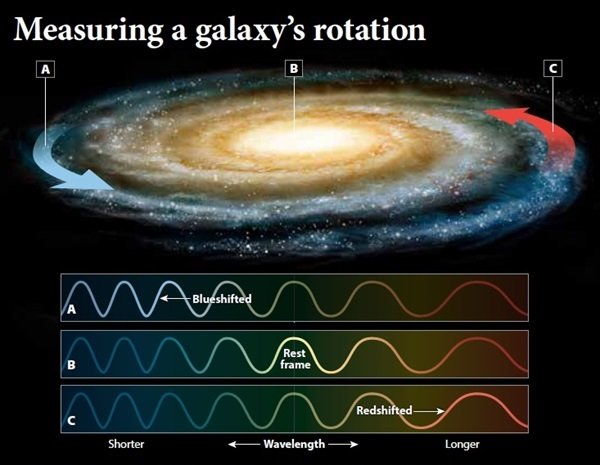
\includegraphics[width=0.5\textwidth,height=0.2\textheight]{Images/GalaxyRotation.jpg}
  \caption{Fig 2. Rotation Curve of a Galaxy}
  \caption{\tiny Source : \url{https://physicsopenlab.org/2020/09/08/measurement-of-the-milky-way-rotation/}}
\end{figure}
\subsubsection{In Cosmology} %subsubsection 2
The 21cm hydrogen line could be used in cosmology to probe the ``dark ages'' of the Universe, i.e., the period from recombination to reionisation. \linebreak
The hydrogen line from that epoch is highly red-shifted and obtained in the frequency range of 200MHz to 9MHz on Earth. \linebreak

We can obtain a picture of how the reionisation occured via this information, as we should obtain holes in the 21cm background spectrum from that epoch which correspond to hydrogen atoms which got ionised by the radiation from stars or quasars.
%%%%%%%%%%%%%%%%%%%%%%%%%%%%%%%%%%%%%%%%%%%%%%%%%%%%%%%%%%%%%section - WAVEGUIDES
\section{Waveguides}
Before building an antenna, we need to first talk about waveguiding structures. 
%subsection - What Are Waveguides?
\subsection{What Are Waveguides?}
Waveguides are structures which can guide waves, like sound waves or electromagnetic waves in a particular direction with minimal loss in energies. \linebreak

Waveguides for electromagnetic waves are made up of hollow metallic (conducting) tubes. They can carry high frequency radio waves. \linebreak

They can be of several types, namely circular, rectangular, elliptical, ridged etc. 
\begin{figure}[H]
  \centering
  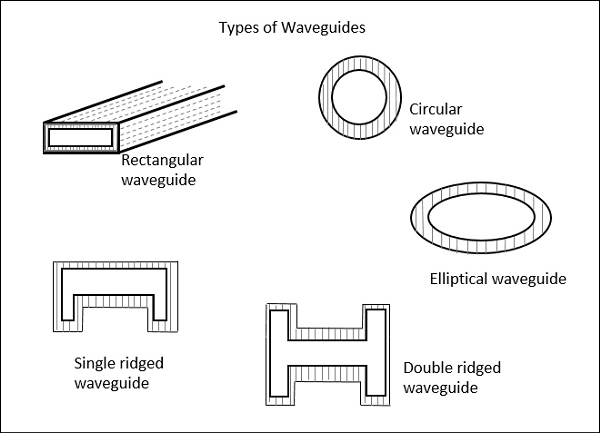
\includegraphics[width=0.5\textwidth]{Images/types_of_waveguides.jpg}
  \caption{Fig 3. Types of Waveguides}
  \caption{\tiny Source : \url{https://www.tutorialspoint.com/microwave_engineering/microwave_engineering_waveguides.htm}}
\end{figure}
%subsection - Arbitrary Waveguide
\subsection{Arbitrary Waveguide}
Let us consider a waveguide with some arbitrary cross section.
\begin{figure}[H]
  \centering
  \includegraphics[width=0.4\textwidth]{Images/arbitrary_waveguide.jpg}
  \caption{Fig 4. Arbitrary Waveguide Structure}
\end{figure}
Let's consider z to be the longitudinal direction, and x-y to be the transverse directions. Writing the EM waves :
\begin{align*}
  \vec{E}&=\vec{E}_{\perp}+E_z \hat{z} \, , \qquad \vec{E}_{\perp}=E_x \hat{x}+E_y \hat{y} \\
  \vec{H}&= \vec{H}_{\perp} + H_z \hat{z} \, , \qquad \vec{H}_{\perp} = H_x \hat{x}+H_y \hat{y} 
\end{align*}
We know from Maxwell's equation :
\begin{equation}
  \nabla \times \vec{E} = -j\omega \mu \vec{H} \label{eq:2}
\end{equation}
where, $\mu$ is the permeability of the space. \linebreak
Using the forms of EM waves written above :
\begin{align*}
  & \left( \nabla_{\perp}+\dfrac{\partial}{\partial z} \hat{z} \right) \times \left( \vec{E}_{\perp}+E_z \hat{z} \right) = -j\omega \mu \left( \vec{H}_{\perp}+ H_z \hat{z} \right) \\
  \implies & \nabla_{\perp} \times E_{\perp} + \nabla_{\perp}\times \left( E_z \hat{z} \right) +\dfrac{\partial}{\partial z}\hat{z}\times \vec{E}_{\perp} + \cancelto{0}{\dfrac{\partial}{\partial z} \hat{z}\times \left( E_z \hat{z}\right)} = -j\omega \mu \left( \vec{H}_{\perp}+H_z \hat{z}\right)
\end{align*}
The last term on LHS goes to zero as it involves the cross product of two parallel vectors. \linebreak
We can also see that the first term on LHS is along z direction, and the second and third terms are transverse terms. Equating the transverse components we obtain :
\begin{equation}
  \vec{H}_{\perp}=-\dfrac{1}{j\omega \mu} \left\{ \nabla_{\perp} \times \left( E_z \hat{z} \right) + \dfrac{\partial}{\partial z} \hat{z}\times \vec{E}_{\perp} \right\} \label{eq:3}
\end{equation}
Similarly, using the other Maxwell's equation :
\begin{equation}
  \nabla \times \vec{H} = j\omega \varepsilon \vec{E} \label{eq:4}
\end{equation}
where, $\epsilon$ is the permittivity of the space. \linebreak
We obtain the transverse component of electric field as :
\begin{equation}
  \vec{E}_{\perp} = \dfrac{1}{j\omega \varepsilon} \left\{ \nabla_{\perp}\times \left( H_z \hat{z} \right)+\dfrac{\partial}{\partial z}\hat{z}\times \vec{H}_{\perp} \right\} \label{eq:5}
\end{equation}
Now substituting for $\vec{H}_{\perp}$ from (\myref{eq:3}) in (\myref{eq:5}) :
\begin{equation*}
  \omega^2 \mu \varepsilon - \dfrac{\partial}{\partial z} \hat{z}\times \dfrac{\partial}{\partial z} \hat{z} \times \vec{E}_{\perp} = -j\omega \mu \nabla_{\perp} \times \left( H_z \hat{z} \right)+\left( \dfrac{\partial}{\partial z}\hat{z} \right) \times \nabla_{\perp} \times \left( E_z \hat{z} \right)
\end{equation*}
Using the triple product identity :
\begin{equation*}
  \vec{A}\times \vec{B}\times \vec{C}=\left( \vec{A}.\vec{C} \right)\vec{B}-\left( \vec{A}.\vec{B} \right)\vec{C}
\end{equation*}
We simplify the triple product terms in the equation above :
\begin{align*}
  \dfrac{\partial}{\partial z}\hat{z}\times \dfrac{\partial}{\partial z} \hat{z} \times \vec{E}_{\perp} &= - \dfrac{\partial^2}{\partial z^2}\vec{E}_{\perp} \\
  \dfrac{\partial}{\partial z}\hat{z}\times \nabla_{\perp}\times E_z \hat{z} &= \nabla_{\perp} \left( \dfrac{\partial E_z}{\partial z} \right)
\end{align*}
The final equation now becomes :
\begin{equation}
  \omega^2 \mu \varepsilon \vec{E}_{\perp} +\dfrac{\partial^2}{\partial z^2}\vec{E}_{\perp} = -j\omega \mu \nabla_{\perp}\times \left( H_z \hat{z} \right)+\nabla_{\perp} \left( \dfrac{\partial E_z}{\partial z} \right) \label{eq:6}
\end{equation}
The Maxwell's equations have only two independent components. Thus, we can choose the z-component of the electric and magnetic fields as the two independent components. So, (\myref{eq:6}) gives us how the transverse electric field depend on the independent components $E_z$ and $H_z$. \linebreak

Taking a travelling wave antasz along the z direction :
\begin{equation}
  E\, , H \sim \exp(-\gamma z) \label{eq:7}
\end{equation}
$\gamma$ is called the absorption coefficient. \linebreak

We ignore solutions for waves travelling in negative direction after reflection by assuming the waveguide is of infinite length. \linebreak
Given the ansatz in (\myref{eq:7}), we can write :
\begin{equation*}
  \dfrac{\partial}{\partial z} \equiv -\gamma \, , \quad \dfrac{\partial^2}{\partial z^2} \equiv \gamma^2
\end{equation*}
Using this in (\myref{eq:6}) :
\begin{equation*}
  \left( \omega^2 \mu \varepsilon+\gamma^2 \right) \vec{E}_{\perp} = -j\omega \mu \nabla_{\perp} \times \left( H_z \hat{z} \right)-\gamma \nabla_{\perp} E_z
\end{equation*}
We can define :
\begin{equation}
  \omega^2\mu \varepsilon+\gamma^2 = h^2 \label{eq:8}
\end{equation}
$h$ is the propagation constant for the transverse wave. \linebreak

Using this, we get the final form for the transverse electric and magnetic fields as :
\begin{align}
  \vec{E}_{\perp} &= -\dfrac{j \omega \mu}{h^2} \nabla_{\perp} \times \left( H_z \hat{z} \right) - \dfrac{\gamma}{h^2}\nabla_{\perp} E_z \label{eq:9}\\
  \vec{H}_{\perp} &= \dfrac{j\omega \varepsilon}{h^2}\nabla_{\perp} \times \left( E_z \hat{z} \right)-\dfrac{\gamma}{h^2} \nabla_{\perp} H_z \label{eq:10}
\end{align}
Since we have chosen the z-components of electric and magnetic fields as the independent components, we can find the complete solutions for the wave motion if we can determine $E_z$ and $H_z$. \linebreak

For a medium that is lossless, 
\begin{equation}
  \gamma = j \beta \label{eq:11}
\end{equation}
We can conclude that :
\begin{enumerate}[i.)]
  \item $E_z$ and $H_z$ both cannot be zero, unless h is zero. Converse is also true. This implies that if both the longitudinal components are zero, there is no transverse wave propagation in the waveguide. EM wave travels as if it is in free space. 
  \item The above mode is called the TEM mode, i.e., Transverse Electric and Magnetic field mode. It is a non-dispersive mode.
  \item When $E_z=0$ and $H_z \neq 0$, it is called the TE mode, i.e., the Transverse Electric mode. It is dispersive mode. 
  \item When $E_z \neq 0$ and $H_z=0$, it is called the TM mode, i.e., the Transverse Magnetic mode. It is a dispersive mode.
\end{enumerate}
%subsection - Rectangular Waveguides
\subsection{Rectangular Waveguides}
A rectangular waveguide is one of the most common types of waveguides used. 
\begin{figure}[H]
  \centering
  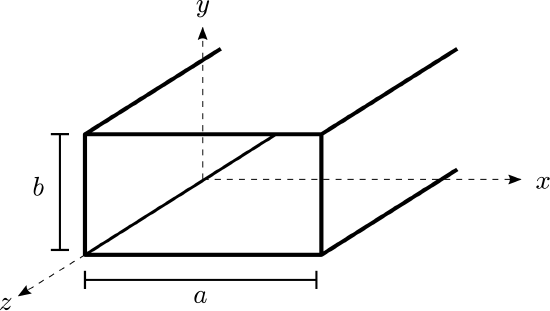
\includegraphics[width=0.5\textwidth]{Images/rectangular.png}
  \caption{Fig 5. Rectangular Waveguide}
  \caption{\tiny Source : \url{https://www.tutorialspoint.com/microwave_engineering/microwave_engineering_waveguides.htm}}
\end{figure}
Let us consider the electromagnetic waves moving along z-direction. \linebreak
We will also assume that for this structure $a\geq b$.\linebreak
\subsubsection{TM Mode} %subsubsection - TM Mode
We will first consider the solutions of TM Mode, i.e.,
\begin{equation*}
  E_z\neq 0 \, , \quad H_z=0
\end{equation*}
Writing the wave equation for electric field travelling in z-direction :
\begin{align*}
  & \nabla^2 E_z + \omega^2 \mu \varepsilon E_z =0 \\
  \implies & \dfrac{\partial^2 E_z}{\partial x^2}+\dfrac{\partial^2 E_z}{\partial y^2}+\dfrac{\partial^2 E_z}{\partial z^2}+\omega^2 \mu \varepsilon E_z=0 
\end{align*}
Applying separation of variables :
\begin{equation*}
  E_z(x,y,z) = X(x)Y(y)Z(z) 
\end{equation*}
Putting this in the wave equation, we obtain the final solution as :
\begin{align*}
  X(x)&= c_1 \cos(Ax)+c_2 \sin(Ax) \\
  Y(y)&= c_3 \cos(By)+c_4 \sin(By) \\
  Z(z)&= c_5 \exp(-j \beta z)+c_6 \exp(j \beta z)
\end{align*}
The solutions $X(x)$ and $Y(y)$ are standing wave solutions. The solution $Z(z)$ is the travelling wave solution.\linebreak

As we had assumed earlier that the waveguide we are using is of infinite length, and there is no reflected wave (wave travelling in -z direction), we can write $c_6=0$. \linebreak

Now using the four boundary conditions due to the four walls upon which $E_z$ is tangential, i.e.,
\begin{equation*}
  E_z = 0 \quad \text{ for } \quad x=0\, , \quad x=a \, , \quad y=0 \, , \quad y=a
\end{equation*}
we obtain the constants $A$ and $B$ as :
\begin{equation}
  A=\dfrac{m\pi}{a} \, , \quad B=\dfrac{n\pi}{b} \label{eq:12}
\end{equation}
We obtain the final solution for $E_z$ as :
\begin{equation}
  E_z = C \sin\left( \dfrac{m\pi}{a}x \right)\sin\left( \dfrac{n\pi}{b}y \right)\exp\left( -j\beta z \right) \label{eq:13}
\end{equation}
Now using the expression for $E_z$ (\myref{eq:13}) in (\myref{eq:9}) and (\myref{eq:10}), we obtain the transverse wave equations as :
\begin{align}
  E_x &= -\dfrac{j \beta}{h^2}\dfrac{\partial E_z}{\partial x} = -\dfrac{j \beta}{h^2}\left( \dfrac{m\pi}{a} \right) C \cos \left( \dfrac{m \pi x}{a} \right) \sin\left( \dfrac{n\pi y}{b} \right) \exp(-j\beta z) \label{eq:14} \\
  E_y &= -\dfrac{j \beta}{h^2}\dfrac{\partial E_z}{\partial y} = -\dfrac{j \beta}{h^2} \left( \dfrac{n\pi}{a} \right) C \sin\left( \dfrac{m\pi x}{a} \right)\cos\left( \dfrac{n\pi y}{b} \right) \exp(-j\beta z) \label{eq:15} \\
  H_x &= \dfrac{j\omega \varepsilon}{h^2} \dfrac{\partial E_z}{\partial y} = \dfrac{j \omega \varepsilon}{h^2}\left( \dfrac{n\pi}{b} \right) C\sin\left( \dfrac{m\pi x}{a} \right) \cos\left( \dfrac{n\pi y}{b} \right)\exp(-j\beta z) \label{eq:16} \\
  H_y &= -\dfrac{j\omega \varepsilon}{h^2} \dfrac{\partial E_z}{\partial x} = -\dfrac{j \omega \varepsilon}{h^2} \left( \dfrac{m\pi}{a} \right)C \cos\left( \dfrac{m\pi x}{a} \right)\sin\left( \dfrac{n\pi y}{b} \right) \exp(-j\beta z) \label{eq:17}
\end{align}
The conclusions we can immediately draw from the above equations are as follows :
\begin{enumerate}[i.)]
  \item The TM\textsubscript{00} mode does not exist. All the waves become zero. 
  \item If either $m=0$ or $n=0$, then also none of the components exist. Thus, TM\textsubscript{m0} and TM\textsubscript{0n} modes also do not exist.
  \item TM\textsubscript{11} is the lowest TM mode that can exist in the rectangular waveguide.
\end{enumerate}
Also, from (\myref{eq:8}), (\myref{eq:11}) and the separable solutions, we can write :
\begin{equation}
  h^2=\omega^2 \mu \varepsilon -\beta^2 = A^2+B^2 = \left( \dfrac{m\pi}{a} \right)^2 + \left( \dfrac{n \pi}{b} \right)^2 \label{eq:18}
\end{equation}
\subsubsection{TE Mode} %subsubsection - TE Mode
Now considering the TE Mode, i.e.,
\begin{equation*}
  E_z=0 \, , \quad H_z \neq 0
\end{equation*}
We need to first solve for $H_z$, as we did for the case of TM mode. \linebreak
After following the similar procedure, we obtain the form of $H_z$ as :
\begin{equation}
  H_z = C \cos\left( \dfrac{m\pi x}{a} \right)\cos\left( \dfrac{n\pi y}{a} \right) \exp(-j\beta z) \label{eq:19}
\end{equation}
We can analyse the above equation directly to look for possible lowest order modes.
\begin{enumerate}[i.)]
  \item For $m=n=0$, $H_z$ is a constant. It does not vary with time. So, all transverse components of the field is zero, i.e., $\vec{E}_{\perp}=\vec{H}_{\perp}=0$. This is because $\vec{E}_{\perp}$ and $\vec{H}_{\perp}$ contain space derivatives of $H_z$. From this we can immediately as $H_z$ must be zero too, as magnetic field cannot exist in the absence of a time-varying electric field. Thus, the TE\textsubscript{00} mode does not exist. 
  \item The TE\textsubscript{m0} and TE\textsubscript{0n} modes exist. Thus the lowest order mode could be either TE\textsubscript{10} or TE\textsubscript{01} mode.
\end{enumerate}
\subsubsection{Cut-off Frequency, Dominant Mode and Field Pattern}





\end{document}